\documentclass[DM,toc]{lsstdoc}

\usepackage{hyperref}
\usepackage{graphicx}

\newcommand{\tblref}[1]{\hyperref[tbl:#1]{#1}}
\widowpenalty=1000
\clubpenalty=1000

\title{The Gen3 Butler Registry Schema}

\author{Jim Bosch}

\setDocRef{DMTN-073}
\date{2018-02-19}
\setDocUpstreamLocation{\url{https://github.com/lsst-dm/dmtn-073}}

\setDocAbstract{%
Documentation for the SQL schema that will be used to manage datasets in the Gen3 Butler.
}

\setDocChangeRecord{%
\addtohist{}{2018-02-19}{Initial version.}{J.~Bosch}
%\addtohist{1}{yyyy-mm-dd}{Future changes}{Future person}
}

\begin{document}

\maketitle

\section{Overview}
\label{sec:overview}

This document is a human-readable description of the minimal SQL schema that will be used in the Gen3 Butler's Registry component.

While some Registry instances may have additional tables, all must provide at least the tables and views described here, and are generally expected to use the mechanisms described here for most extensions.

The normative, machine-readable version of the minimal schema can be found at: \verb`daf_butler:config/registry/default_schema.yaml`.
The tables and figures in this document (including the descriptions of table columns) are generated from the contents of that file.


\section{Datasets}
\label{sec:datasets}

The central table of the registry database is \tblref{Dataset}, which contains one record for every dataset managed by the registry.

\subsubsection*{Dataset}
\label{tbl:Dataset}

{
    \footnotesize
    \begin{tabular}{| l | l | l | p{0.5\textwidth} |}
  \hline
  \textbf{Name} & \textbf{Type} & \textbf{Attributes} & \textbf{Description} \\
  \hline
  dataset\_id & int & PRIMARY KEY &
      A unique autoincrement field used the primary key for dataset.
      \\
  \hline
  dataset\_type\_name & str & NOT NULL &
      The name of the \tblref{DatasetType} associated with this dataset;
      a reference to the \tblref{DatasetType} table.
      \\
  \hline
  run\_id & int & NOT NULL &
      The id of the run that produced this dataset, providing access to
      coarse provenance information.
      \\
  \hline
  quantum\_id & int &  &
      The id of the quantum that produced this dataset, providing access
      to fine-grained provenance information. may be null for datasets
      not produced by running a supertask.
      \\
  \hline
  camera & str &  &
      \\
  \hline
  abstract\_filter & str &  &
      String name for the abstract filter, frequently a single
      character.
      \\
  \hline
  physical\_filter & str &  &
      \\
  \hline
  sensor & str &  &
      \\
  \hline
  visit & int &  &
      \\
  \hline
  exposure & int &  &
      \\
  \hline
  valid\_first & int &  &
      First exposure identifier included in the range (inclusive).  may
      be zero to indicate an open interval.
      \\
  \hline
  valid\_last & int &  &
      Last exposure identifier included in the range (inclusive).  may
      be max(int) to indicate an open interval.
      \\
  \hline
  skypix & int &  &
      Unique id of a pixel in the hierarchical pixelization, using a
      numbering scheme that also encodes the level of the pixel.
      \\
  \hline
  skymap & str &  &
      \\
  \hline
  tract & int &  &
      \\
  \hline
  patch & int &  &
      \\
  \hline
  label & str &  &
      A string value composed only of letters, numbers, and underscores.
      \\
  \hline
\end{tabular}

}

\begin{figure}
    \centering
    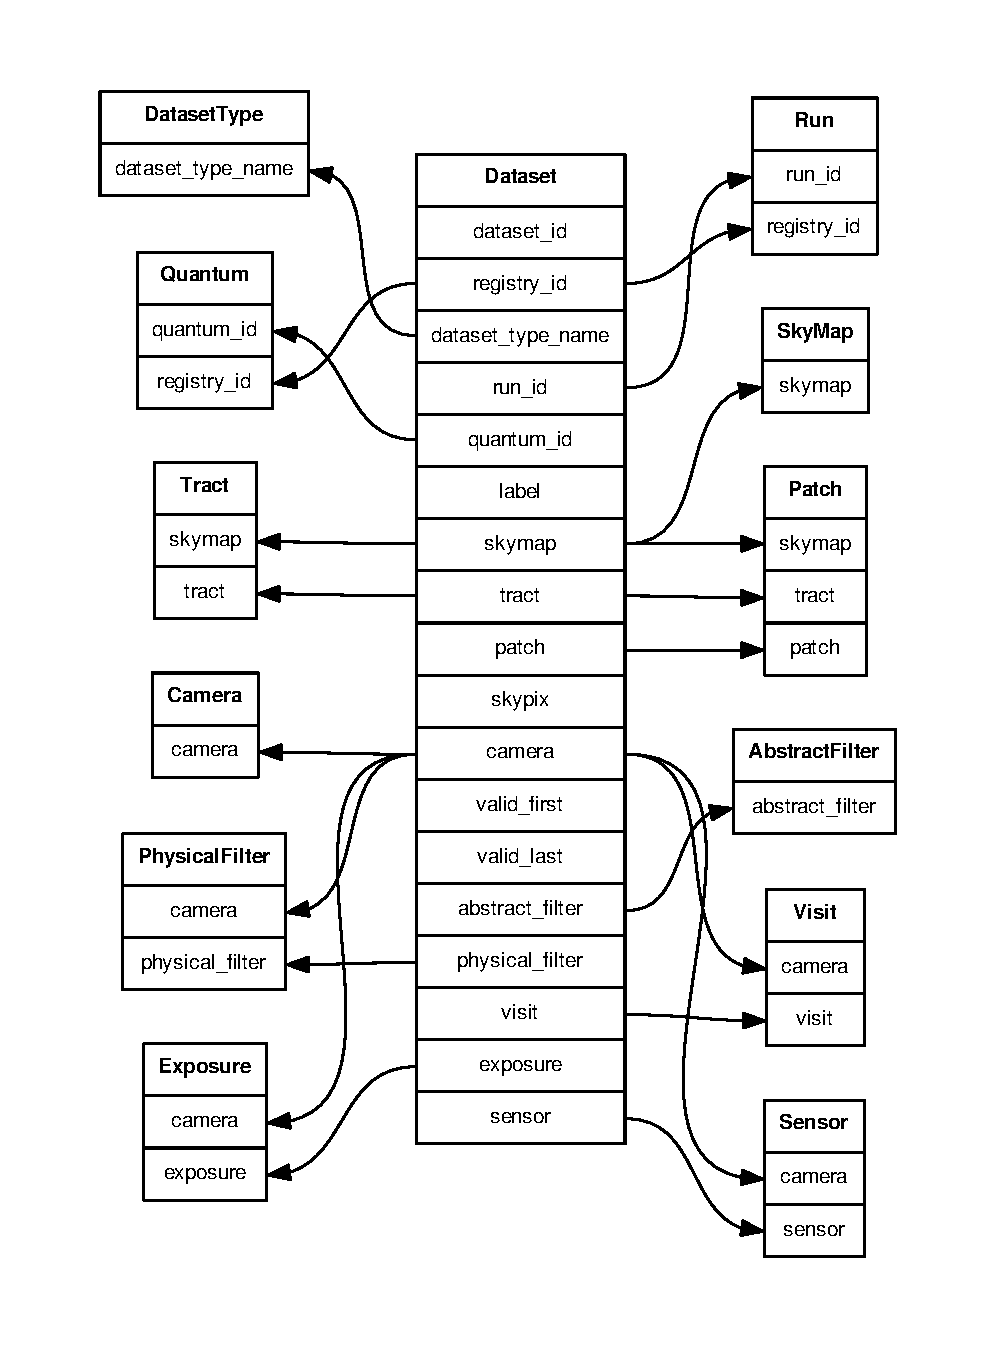
\includegraphics[width=0.8\textwidth]{generated/Dataset_relationships}
    \caption{Dataset Table Relationships}
    \label{rel:Dataset}
\end{figure}

\subsection{DatasetTypes and StorageClasses}
\label{sec:datasettypes-and-storageclasses}

\subsubsection*{DatasetType}
\label{tbl:DatasetType}
{
    \footnotesize
    \begin{tabular}{| l | l | l | p{0.5\textwidth} |}
  \hline
  \textbf{Name} & \textbf{Type} & \textbf{Attributes} & \textbf{Description} \\
  \hline
  dataset\_type\_name & str & PRIMARY KEY &
      Globally unique name for this \tblref{DatasetType}.
      \\
  \hline
  storage\_class & str & NOT NULL &
      Name of the StorageClass associated with this
      \tblref{DatasetType}.  All registries must support the full set of
      standard StorageClasses, so the set of allowed StorageClasses and
      their properties is maintained in the registry Python code rather
      than the database.
      \\
  \hline
\end{tabular}

}

\subsubsection*{DatasetTypeUnits}
\label{tbl:DatasetTypeUnits}
{
    \footnotesize
    \begin{tabular}{| l | l | l | p{0.5\textwidth} |}
  \hline
  \textbf{Name} & \textbf{Type} & \textbf{Attributes} & \textbf{Description} \\
  \hline
  dataset\_type\_name & str & NOT NULL &
      The name of the \tblref{DatasetType}.
      \\
  \hline
  unit\_name & str & NOT NULL &
      The name of a DataUnit associated with this \tblref{DatasetType}.
      \\
  \hline
\end{tabular}

}

\begin{figure}
    \centering
    \includegraphics[width=0.8\textwidth]{generated/DatasetTypeUnits_relationships}
    \caption{DatasetTypeUnits Table Relationships}
    \label{rel:DatasetTypeUnits}
\end{figure}


\subsection{Composite Datasets}
\label{sec:composite-datasets}


\section{DataUnits}
\label{sec:dataunits}

\subsection{Fundamental DataUnits}
\label{sec:fundamental-dataunits}

\subsection{Camera DataUnits}
\label{sec:camera-dataunits}

\subsection{SkyMap DataUnits}
\label{sec:skymap-dataunits}

\subsection{Joins Between DataUnits}
\label{sec:joins-between-dataunits}


\section{Collections and Provenance}
\label{sec:collections-and-provenance}

\subsection{Collections}
\label{sec:collections}

\subsection{Execution}
\label{sec:excution}

\subsection{Run}
\label{sec:run}

\subsection{Quantum}
\label{sec:quantum}


\section{Additional Metadata Tables}
\label{sec:additional-metadata-tables}

\subsection{StorageClass Metadata}
\label{sec:storageclass-metadata}

\subsection{DatasetType Metadata}
\label{sec:datasettype-metadata}

\subsection{DataUnit Metadata}
\label{sec:dataunit-metadata}


\section{Multi-User Environments}
\label{sec:multi-user-environments}

\subsection{Cross-Registry Auto-Increment Keys}
\label{sec:cross-registry-auto-increment-keys}

\subsection{Namespaces for Collections and DatasetTypes}
\label{sec:namespaces-for-collections-and-datasettypes}

\subsection{Combining Layered Databases}
\label{sec:layered-databases}


\end{document}
